\section{CERN and the Large Hadron Collider}
The \textit{organisation européenne pour la recherche nucléaire} or CERN conducts the world's frontier particle physics experiments. It's a coalition of scientists representing numerous countries around the world who work together for a greater understanding of the universe. CERN hosts the Large Hadron Collider, currently the largest particle collider in the world. It is 27 km in circumference and holds eight experimental caverns 150 meters underneath the earth. Accelerator physicists and engineers strive to provide high energy collisions along these eight sites. Monumental effort is made to guide the beam, utilizing more than 1500 superconducting magnets to steer, press, and shape the accelerating protons. Crossing points facilitated by crab cavities force these particles to cross, collide, and interact at the caverns where the experiments take data. Multiple campaigns for particle physics are done such as low intensity fills, lead-lead collisions, and proton collision. The Compact Muon Solenoid (CMS) is the general purpose proton-proton detector located at P5 in Cessy, France that took the data that will be analyzed in this dissertation ~\cite{Bruning:782076}. 

\begin{figure}[ht!b]
  \centering
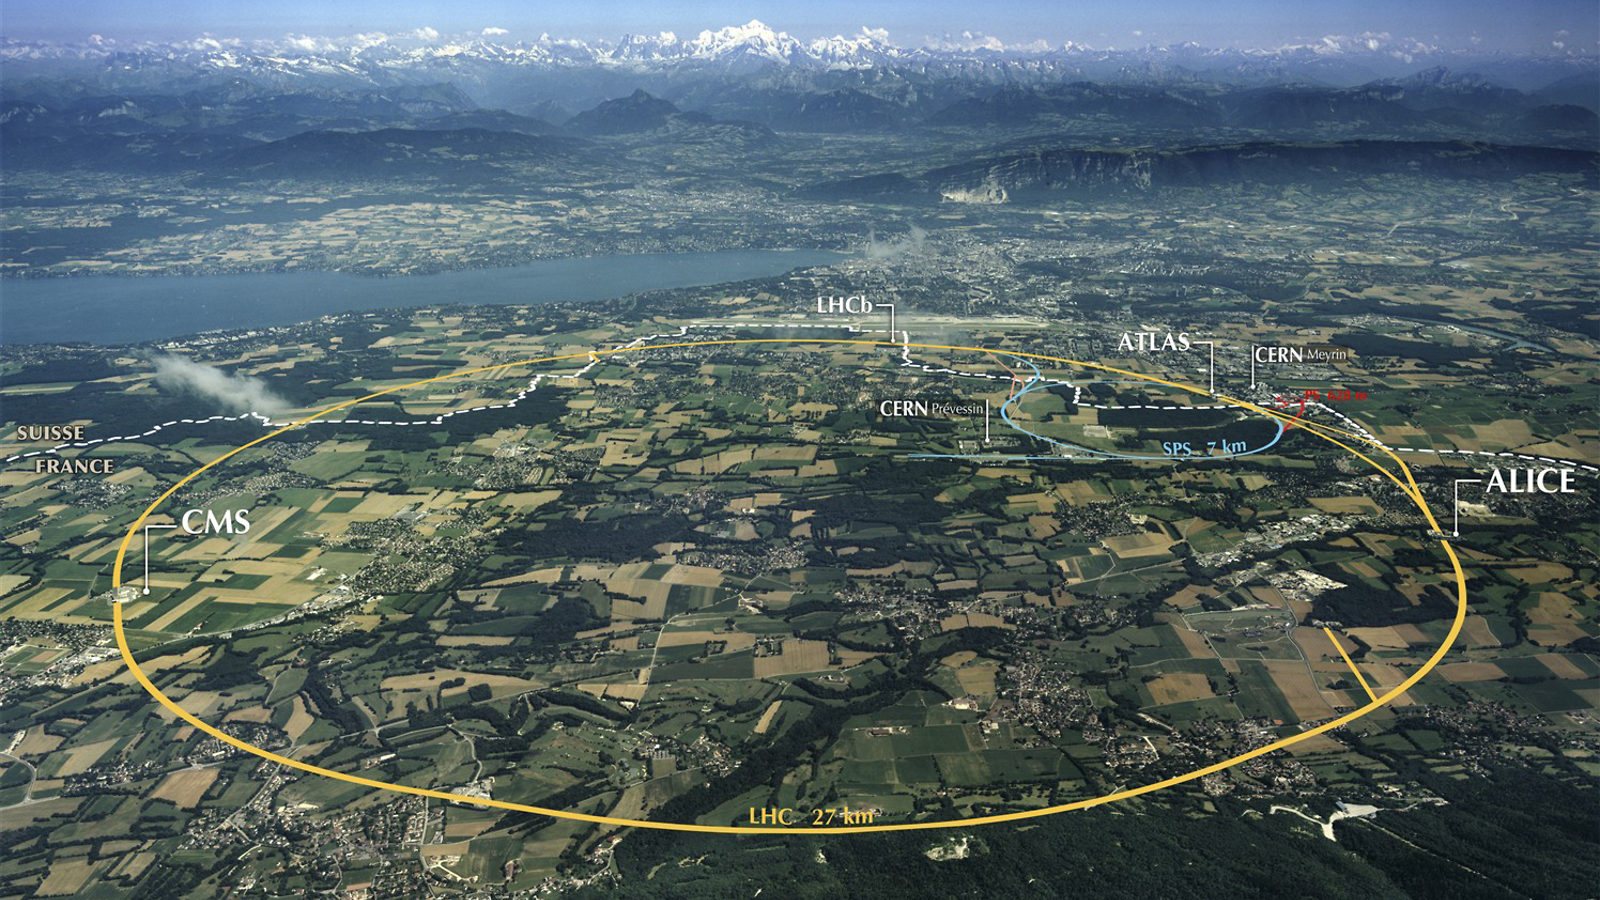
\includegraphics[width=0.75\textwidth]{figures/LHC_map-s.jpg}    
    \caption{\label{fig:lhc} Overview of the Large Hadron Collider spanning Switzerland and France - Maximilien Brice, CERN }
\end{figure}

\section{The Compact Muon Solenoid detector}
At around 14,000 tonnes, the CMS detector may not seem like it would be compact; however, it is quite dense. As shown in the diagram, the detector contains many sub-detector systems and also features the most powerful solenoid magnet ever made for its size. At 6 meters inner diameter, and a combined weight of the solenoid and the steel return yolk of 12,500 tonnes, the solenoid is the central feature of the Compact Muon Solenoid (CMS) \ref{fig:cmsdet}.
\begin{figure}[!htb]
\begin{center}
\includegraphics[width=0.75\textwidth]{Figures/cmsDet.png}
\caption{\label{fig:cmsdet}The CMS detector full 3D image with all subsystems labeled}
\end{center}
\end{figure}
 Within the solenoid volume, there is the
silicon pixel and strip tracker, a lead tungstate crystal 
electromagnetic calorimeter (ECAL), and a brass plus scintillator 
hadron calorimeter (HCAL). Each tracker and calorimeter is composed of a barrel and two endcap 
sections. Forward calorimeters extend the pseudorapidity---$\eta$---
coverage provided by the barrel and endcap detectors. 
Muons are detected in gas-ionization chambers embedded 
in the steel flux-return yoke outside the solenoid.

The coordinate system that is adopted is cylindrical in nature starting at the interaction or nominal collision point. The $y$-axis points vertically outward toward the sky, the $x$-axis tangent to the Earth, and the $z$-axis along the direction of the beam pipe. The azimuthal angle $\phi$ and the radial coordinate $r$ in the $x$ and $y$ plane, and the polar angle $\theta$ measured from the $z$ axis comprise the angular coordinate interpretation. Often pseudorapidity is used to describe angular distance from the beam pipe---useful in detector segmentation in forward and barrel regions:
\begin{equation}\eta = - \ln \tan(\theta/2)\end{equation}  


%From the central interaction point, the CMS detector hosts
%the silicon pixel and strip tracker, the lead tungstate crystal electromagnetic
%calorimeter (ECAL), and the brass-scintillator hadron calorimeter (HCAL),
%each composed of a barrel and two endcap sections. The silicon pixel and tracking systems as well as
%the calorimeters are contained within the solenoid volume.  %cite

%The nominal $\Pp\Pp$ bunch crossing rate at the LHC is 40\unit{MHz}. This rate would be too extreme for any data taking system. In order to reduce the rate of events that are recorded for offline analysis, events of interest are selected using a two-step trigger system~\cite{Khachatryan:2016bia}.
%The first level (L1) is composed of custom built electronics which makes use of
%high speed optical links and large Field Programmable Gate Arrays (FPGAs). 

%L1 reduces the event rate from the nominal bunch crossing to a rate of aroun 100\unit{kHz} within a time interval of less than 3.5\mus.
%L1 reduces the rate from 40 MHz to 100 kHz.

%The second level, known as the High Level Trigger (HLT), consists of a farm of 
%generic processors running a version of the full event reconstruction software that
% has been optimized for fast processing. The HLT reduces the event rate to about
%1\unit{kHz} before data storage.

%Since the 2012 data taking, significant upgrades of the L1 trigger 
%have benefited this analysis, especially in the final state with two semi-hadronically decaying 
%$\Pgt$ leptons, denoted as $\tauh$.  
%These upgrades improved the $\tauh$ identification at L1 by giving more flexibility 
%to object isolation, allowing new techniques to suppress the contribution from 
%additional $\Pp\Pp$ interactions per bunch
%crossing, and to reconstruct the L1 $\tauh$ object in a fiducial region that matches 
%more closely that of a true $\tauh$ decay.

A more detailed description of the CMS detector can be found in Reference ~\cite{Chatrchyan:2008zzk}.

%In Phase 2, many upgrades are planned after Run III---which is currently on-going. 


\section{Subdetector Systems}
Several subdetector systems play an important role in the identification of muons and tau leptons that are used in the analysis. Some impressive infrastructure that supports physics at CMS and physicists worldwide will also be described. 
While all subdetector systems are important to event reconstruction in CMS, there are several detectors that contribute to the particles that are identified in the pseudoscalar search. These are the tracker system, electromagnetic calorimeter, the hadronic calorimeter, and muon system. 

\subsection{Tracker}
Working around silicon for almost 10 years, I have a slight bias in presenting this sub-detector system and I plan to share more details in this section than others. 

The tracker comprises several groups of silicon detectors. 


Going outward from the beam pipe and central interaction points, there is the pixel detector system and then the silicon tracker system. For better coverage, both are divided into barrel and endcap components. 

A silicon detector is a detector that can identify charge by disturbing the electron lattice that exists on the silicon itself. 
Typically, multiple band gaps are created through the process of lithography which adds artificial impurities of p-type (holes) or n-type (electrons). This process is known as ``doping". When a minimum ionizing particle (MIP) disturbs the latent charge---set by the bias voltage on the sensor---there is a current generated in the n and p type components (Shockley Equation):
\begin{equation}
\label{eq:shockleyn}
\mathcal{J}_{n,p} = \frac{q_0 D_{n,p} d_{n,p}}{L_{n,p}}\left(e^{\frac{q_0 V}{k_B T}} - 1 \right)
\end{equation}
For reference, $L_{n,p}$ is the diffusion length, $D_{n,p}$ the diffusion coefficients, $d_{n,p}$ the charge/hole density, $V$ the bias voltage, $q_0$ the standard charge unit, $k_B$ the Boltzmann constant, and $T$ the temperature. 
This sets in motion the current which will be collected later by each of the channels. A graphical display of surface current dissipation using TCAD (technology computer aided design) as a function of time can be displayed in figure \ref{fig:sd}. A wealth of silicon information can be found in reference ~\cite{Eichhorn:2112017}.

\begin{figure}[ht!b]
  \centering
  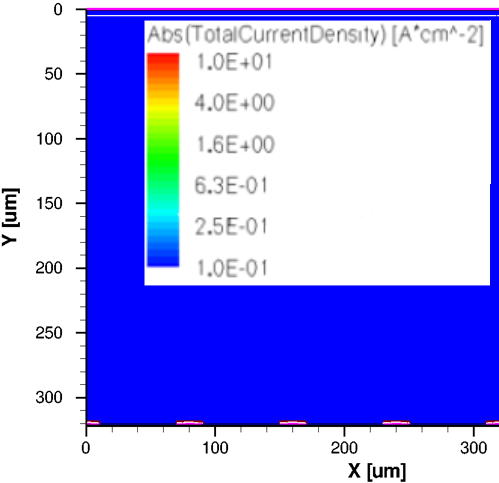
\includegraphics[width=0.31\textwidth]{figures/silicon/silicon_t0.0.png}
  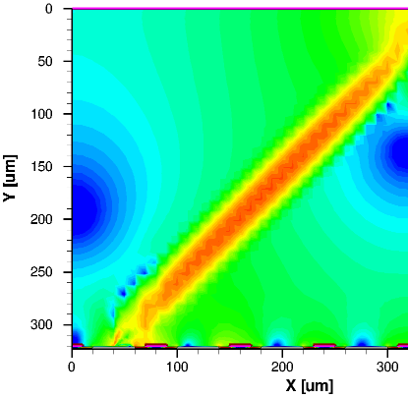
\includegraphics[width=0.31\textwidth]{figures/silicon/silicon_t1.1.png}
  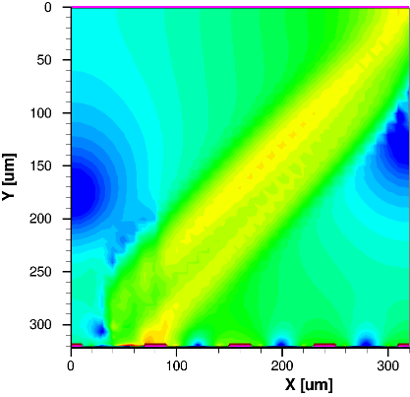
\includegraphics[width=0.31\textwidth]{figures/silicon/silicon_t1.5.png}\\
  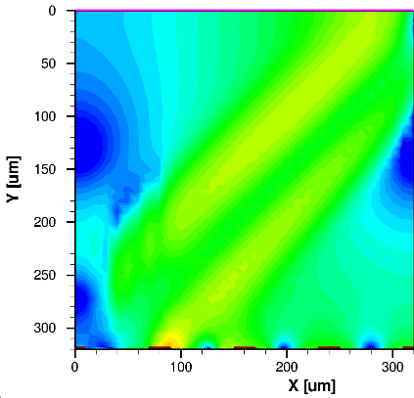
\includegraphics[width=0.31\textwidth]{figures/silicon/silicon_t2.0.png}
  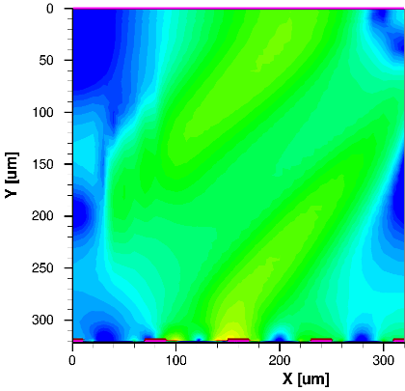
\includegraphics[width=0.31\textwidth]{figures/silicon/silicon_t3.0.png}
  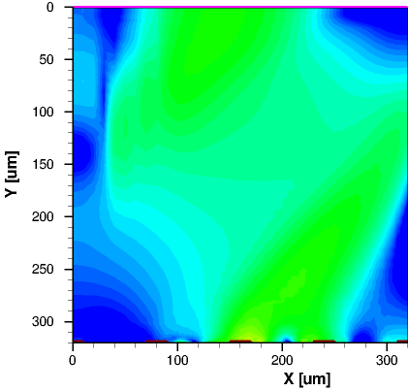
\includegraphics[width=0.31\textwidth]{figures/silicon/silicon_t4.0.png}\\
  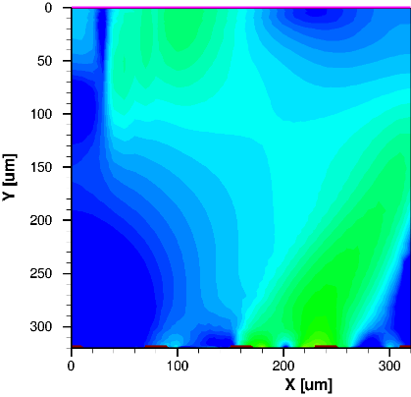
\includegraphics[width=0.31\textwidth]{figures/silicon/silicon_t5.0.png}
  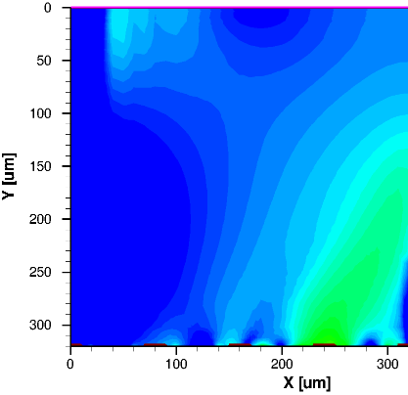
\includegraphics[width=0.31\textwidth]{figures/silicon/silicon_t6.0.png}
  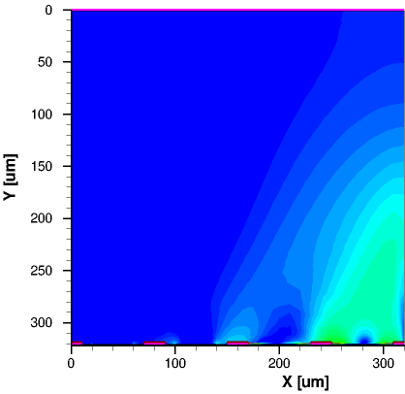
\includegraphics[width=0.31\textwidth]{figures/silicon/silicon_t7.0.png}\\
    \caption{\label{fig:sd} (simulation) MIP particle traveling across a silicon strip sensor at $45^\circ$ over time from 0.0, 1.1,1.5,2,3,4,5,6,7 nanoseconds. The induced surface current dissapates and would be collected by the channels of the silicon module ~\cite{Eichhorn:2112017}.}
\end{figure}





\subsubsection{Pixel Detector}
\label{sec:pixeldet}
Sitting closest to the beam pipe is the pixel detector system. It contains the Barrel Pixels (BPIX) and the Forward Pixel System (FPIX).  
Similar 2x8 silicon detector modules make up both the BPIX and FPIX systems.

In 2016, the phase 1 Forward Pixel System (FPIX) was constructed and tested. At Purdue University, an Aerotech robotic gantry control system was used to join a hybrid flex circuit to a bump-bonded silicon pixel module. After wirebonding, the gantry system encapsulated the wirebonds for protection from corrosion and magnetic field resonance. Purdue was one of the manufacturing sites alongside University Nebraska-Lincoln. 

Using LabVIEW, we developed a state machine to assemble and encapsulate these pixel modules. Pattern recognition and a linear algebra suite were developed to perform precise operations at a 50 micron resolution. An example of a post encapsulated token bit manager - which resides on top of the high density interconnect of a completely assembly module - is shown in figure \ref{fig:tbm}.

\begin{figure}[ht!b]
    \centering
  \includegraphics[width=0.65\textwidth]{fpixtbm.jpg}
    \caption{\label{fig:tbm} encapsulated token bit manager of a forward pixel module currently installed in CMS}
\end{figure}


In 2017, this system was installed in CMS, increasing the number of disks to three and the number of barrel layers to four.  Due to the experimental design of CMS, the inner sub-detector systems may be taken out of the inner body---the solenoid---and serviced.  
These forward disks are especially important for reconstruction of events with boosted charged particles. They are located in high regions of $\eta$ and are overlapped for improved hermeticity.  


\subsubsection{Silicon Tracker}
The silicon tracker comprises larger silicon modules by area than the pixel system and is located further from the beam pipe. A representative layout of the silicon tracker and the pixel system can be found in figure \ref{fig:tracker} ~\cite{Chatrchyan:2008zzk}. 

\begin{figure}[ht!b]
\label{fig:tracker}
  \centering
  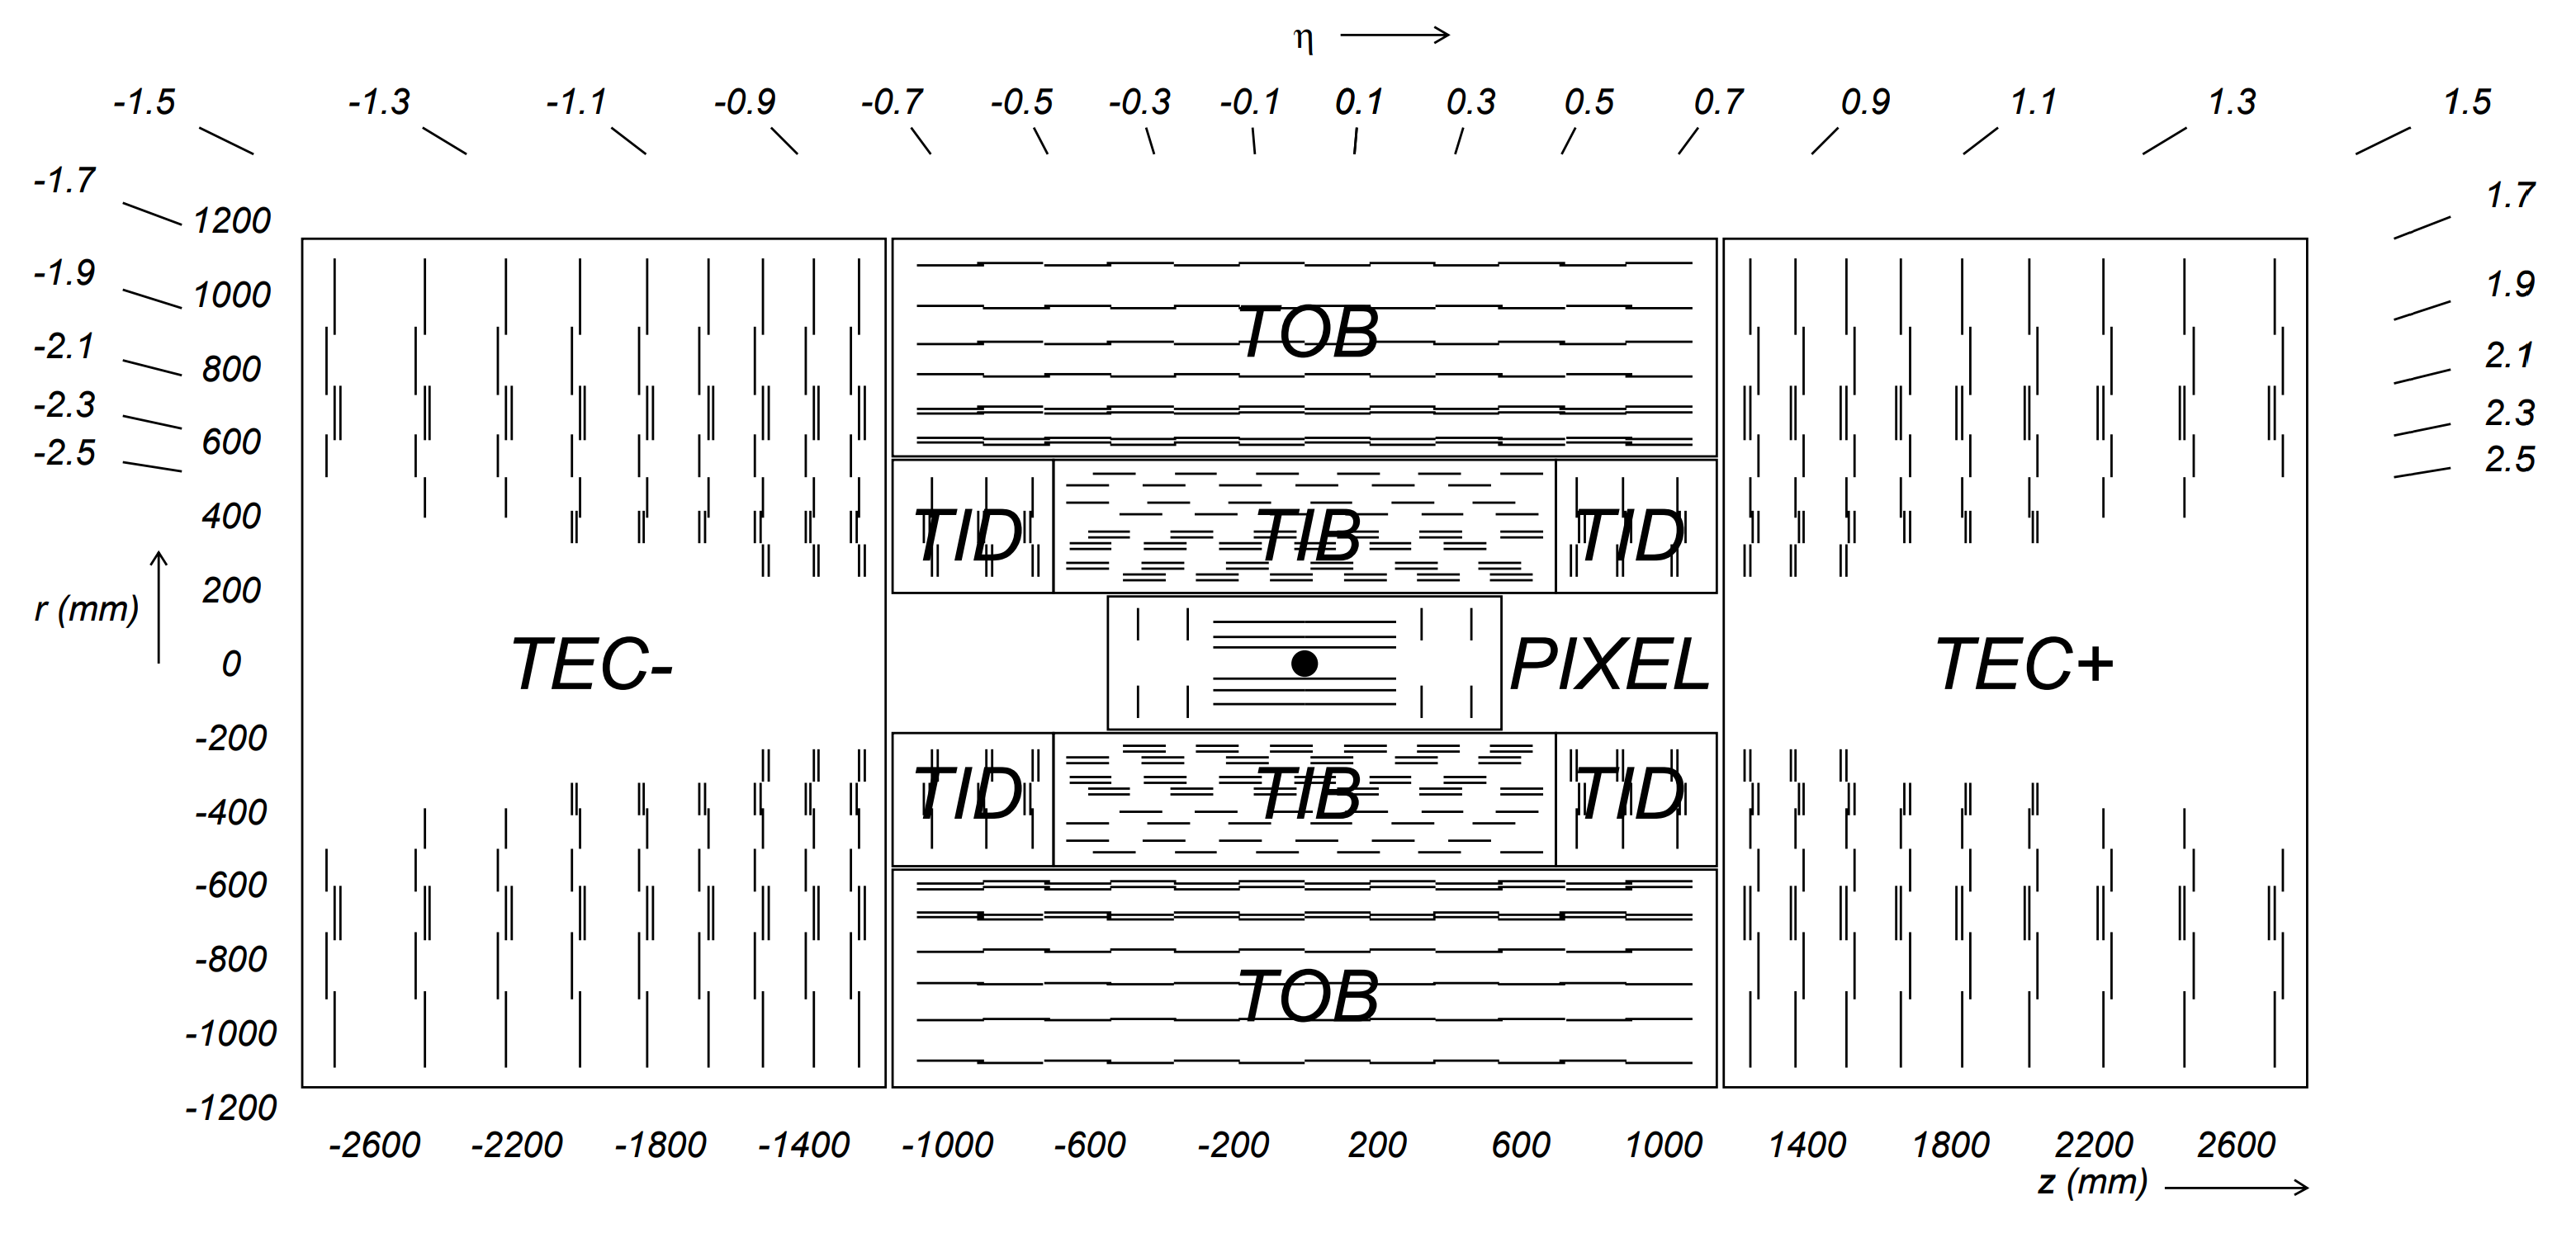
\includegraphics[width=0.85\textwidth]{figures/silicon/SiliconTracker.png}\\
    \caption{ The silicon tracker system, consisting of the inner pixel system (BPIX and FPIX), The Tracker End Caps (TEC), Tracker Inner Detector(TID), Tracker Inner Barrel (TIB), and the Tracker Outer Barrel (TOB) by position in r, z , and $\eta$ ~\cite{Chatrchyan:2008zzk}}
\end{figure}



\subsection{Electronic Calorimeter}

The principal components of the ECAL are the 76200 lead tungstate ($\text{PbWO}_4$) crystals, which scintillate and absorb energy from incoming particles. These detector components are also separated in barrel and endcap regions. Photomultipliers are attached to the crystal to detect the light signal. The relative energy resolution is 
\begin{equation*}
\label{eq:ecal}
\left(\frac{\sigma}{E}\right)^2 = \left( \frac{2.8\%}{\sqrt{E}}  \right)^2 + \left( \frac{0.12}{E}  \right)^2 + (0.3\%)^2 
\end{equation*}
The 2.8\% reflects the stochastic term, 0.12 the Noise term and 0.3\% the constant term in the fit during calibration with a 440 nm blue laser over 11.5 days ~\cite{Chatrchyan:2008zzk,Eichhorn:2112017}. 

\subsection{Hadronic Calorimeter} 
The Hadronic Calorimeter is the primary sub-detector to identify ``jets", which are collections of hadronic processes. These jets have subcomponents of densely clustered energy. 

%Absorber plates are used which cause showers of particles that can be identified through scintillation, similar to the ECAL these signals are read out through photodiodes as well. 
Plates are used to induce particle showers, which can be identified through scintillation. Similar to the ECAL, these signals are read out through photodiodes as well. 

There are barrel (HB) and endcap (HE) inside the solenoid. The Hadronic Outer (H0) and super forward detector (HF) sit outside the solenoid. An overview of the HCAL system is shown in figure \ref{fig:hcal} ~\cite{Chatrchyan:2008zzk,Eichhorn:2112017}. 

\begin{figure}[ht!b]
  \centering
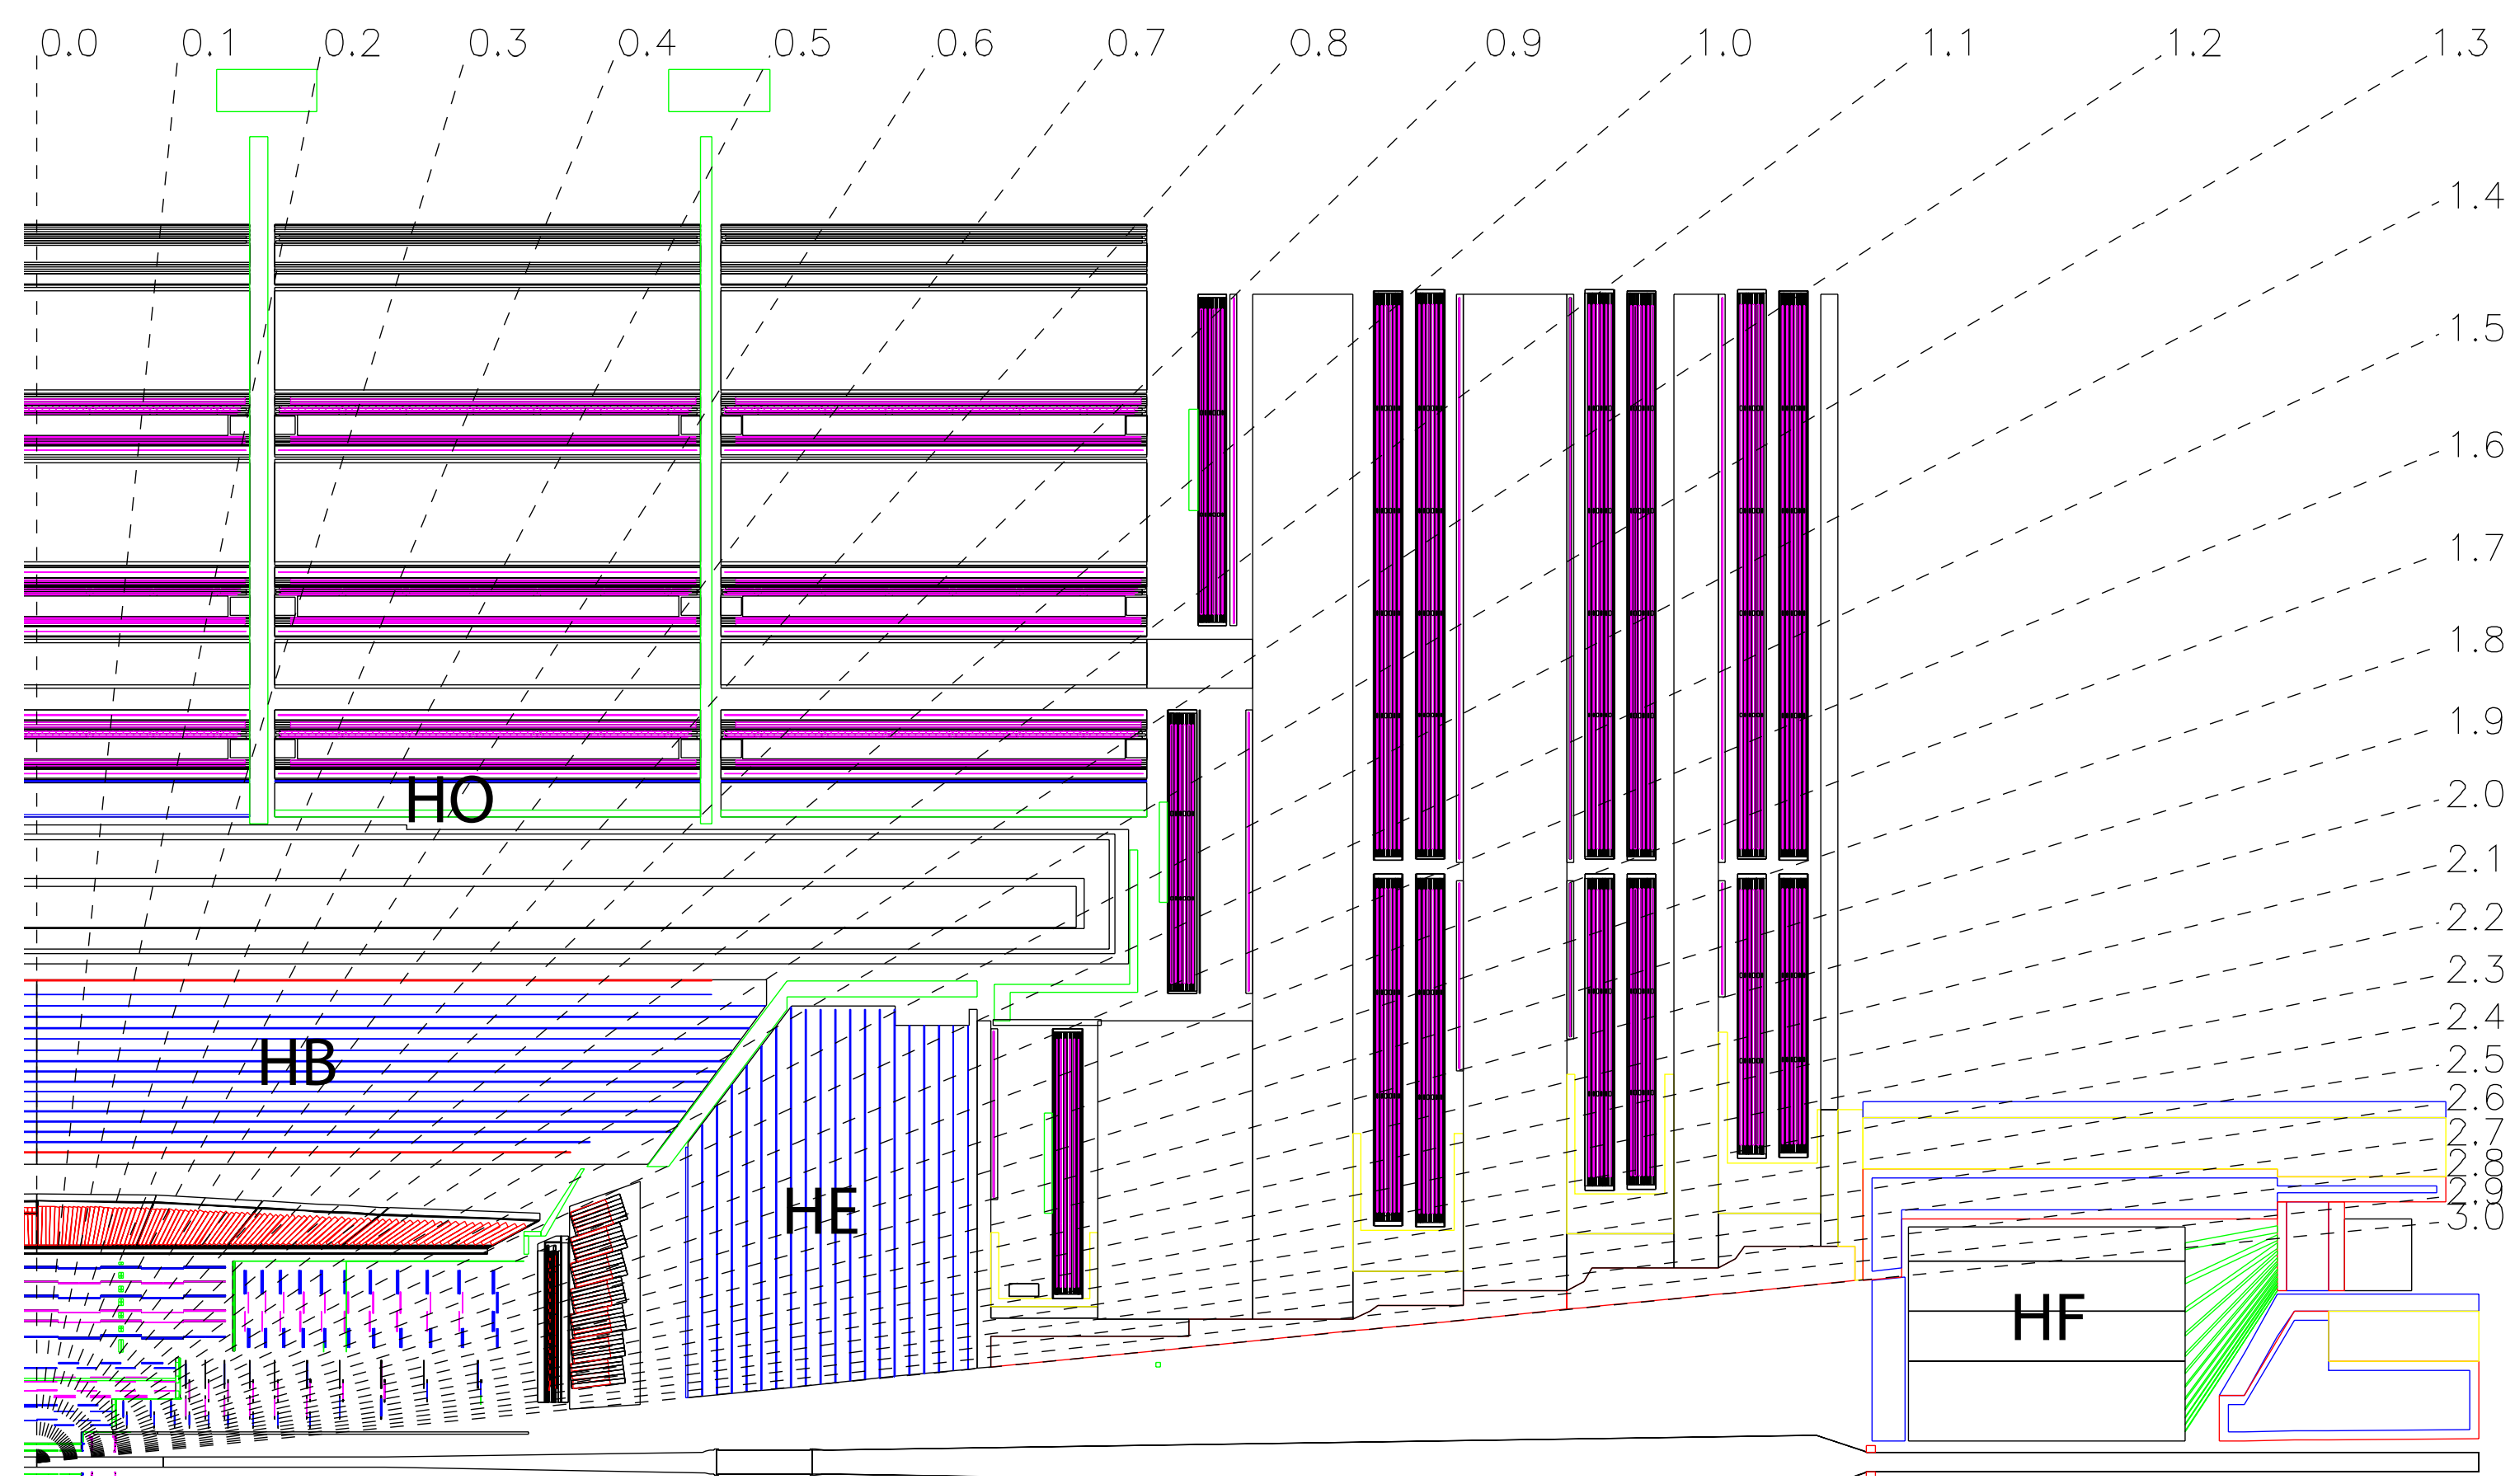
\includegraphics[width=0.85\textwidth]{figures/HCAL.png}    
    \caption{\label{fig:hcal} Overview of the HCAL system from the z---$\eta$ plane showing the hadron barrel (HB), encap(HE), outer (HO), and the forward (HF) subsystems ~\cite{Chatrchyan:2008zzk}}
\end{figure}




\subsection{Muon Chambers} 
The chambers comprises drift tubes which cover a pseudorapidity region ($|\eta|<1.2$) split into 4 stations in the flux return plates.

In the higher $|\eta|$ regions, cathode strip chambers (CSCs) are used and preferred for their fast response time, fine segmentation, and radiation resistance ~\cite{Chatrchyan:1129810}. For a visual representation of a cross section of the muon system please refer to figure \ref{fig:muonsystem}. 

Notably, the track of the muon is bent inside the solenoid by the Lorentz force, and then reverses after it exits. 

\begin{figure}[ht!b]
  \centering
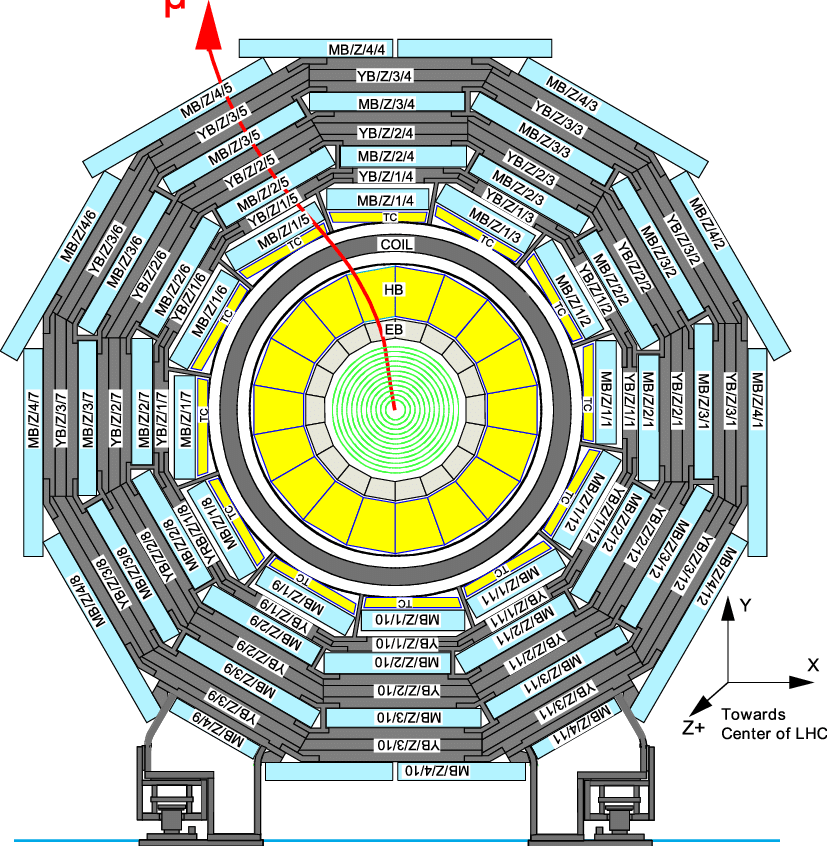
\includegraphics[width=0.75\textwidth]{figures/Layout-of-the-CMS-barrel-muon-DT-chambers-in-one-of-the-5-wheels-59.png}    
    \caption{\label{fig:muonsystem} Muon system involving multiple subtector systems: tracker, solenoid, and the muon gas chambers around the iron yoke (grey) - Maximilien Brice, CERN }
\end{figure}


\section{Level 1 Trigger System and High Level Trigger}
Particle collisions happen at a rate of 40 MHz with 22 minimum bias events expected to occur on average, making full readout impossible to store because of the high bandwidth ~\cite{Bruning:782076,Foudas:2232067}. The Level 1 Trigger System and High Level Trigger work to reduce these rates by recording events that physicists agree are worth saving. 

The Level-1 trigger system can process data close to the beam collision rate. It is the first online event selection that uses many subsystems in tandem to decide whether or not to save the event. Algorithms are in place that take input from the calorimeters, the muon systems, and other detectors in the form of ``trigger primitives'' and use pattern recognition along with fast summing techniques to trigger on the event. Many of these algorithms are run on Field Programmable Gate Arrays (FPGAs). These decisions are concatenated at the CMS Global Trigger (GT) which signals at the front end electronics, 144 beam crossing after the interaction. The Level-1 system also outputs physics objects from the algorithms so preliminary leptons, jets, missing transverse energy among other objects can be used in algorithms operating at the High Level Trigger ~\cite{Foudas:2232067}. 


The HLT maximum input rate is 100KHz and the output is in the order of kHz. It is constrained by the processing power available, the data recording and transfer rate of Tier 0, and the prompt reconstruction algorithms. Late in Run II  ``Scouting'' and ``Parking'' data were used to help increase bandwidth. ``Scouting'' reduces the event size by saving only objects reconstructed at HLT and ``Parking'' avoids prompt reconstruction by saving lower level information ~\cite{Thomas:2703017}.


\section{Particle Flow Algorithms}
The event data model requires association of higher level physics objects---like leptons---with energy deposits and tracks in the detector. 

The particle flow algorithm at CMS has the goal of associating these primary detector signatures with these particles so that direct comparison to Monte Carlo simulation can be done. 

The list includes, but is not limited to jets, missing transverse energy, taus, charged-leptons, photon isolation, and bottom quark jet identification.


To outline the algorithm: Charged particle tracks reconstructed in the tracker, energy clusters from the ECAL, HCAL, and preshower detector (ES), and forward calorimeter (HF) are topologically linked into blocks. The linking is done through many associations of energy deposits and tracks in $\phi,\eta$ space. These blocks are then interpreted as particles and central energies are calibrated depending on their composition. This information and an exhaustive explanation can be found in reference ~\cite{CMS-PAS-PFT-10-001}.

\section{Computational Infrastructure}
Over 200 peta-bytes of information have been gathered in Run II. The way data is gathered, computed, and stored should all be highlighted. 

At CMS above ground there are 32,000 24-core processors at Tier 0 (T0). This is where higher level reconstruction of physics objects is done. A schematic overview of the infrastructure can be found in figure \ref{fig:t0} ~\cite{Hufnagel:1319049}. 

\begin{figure}[ht!b]
  \centering
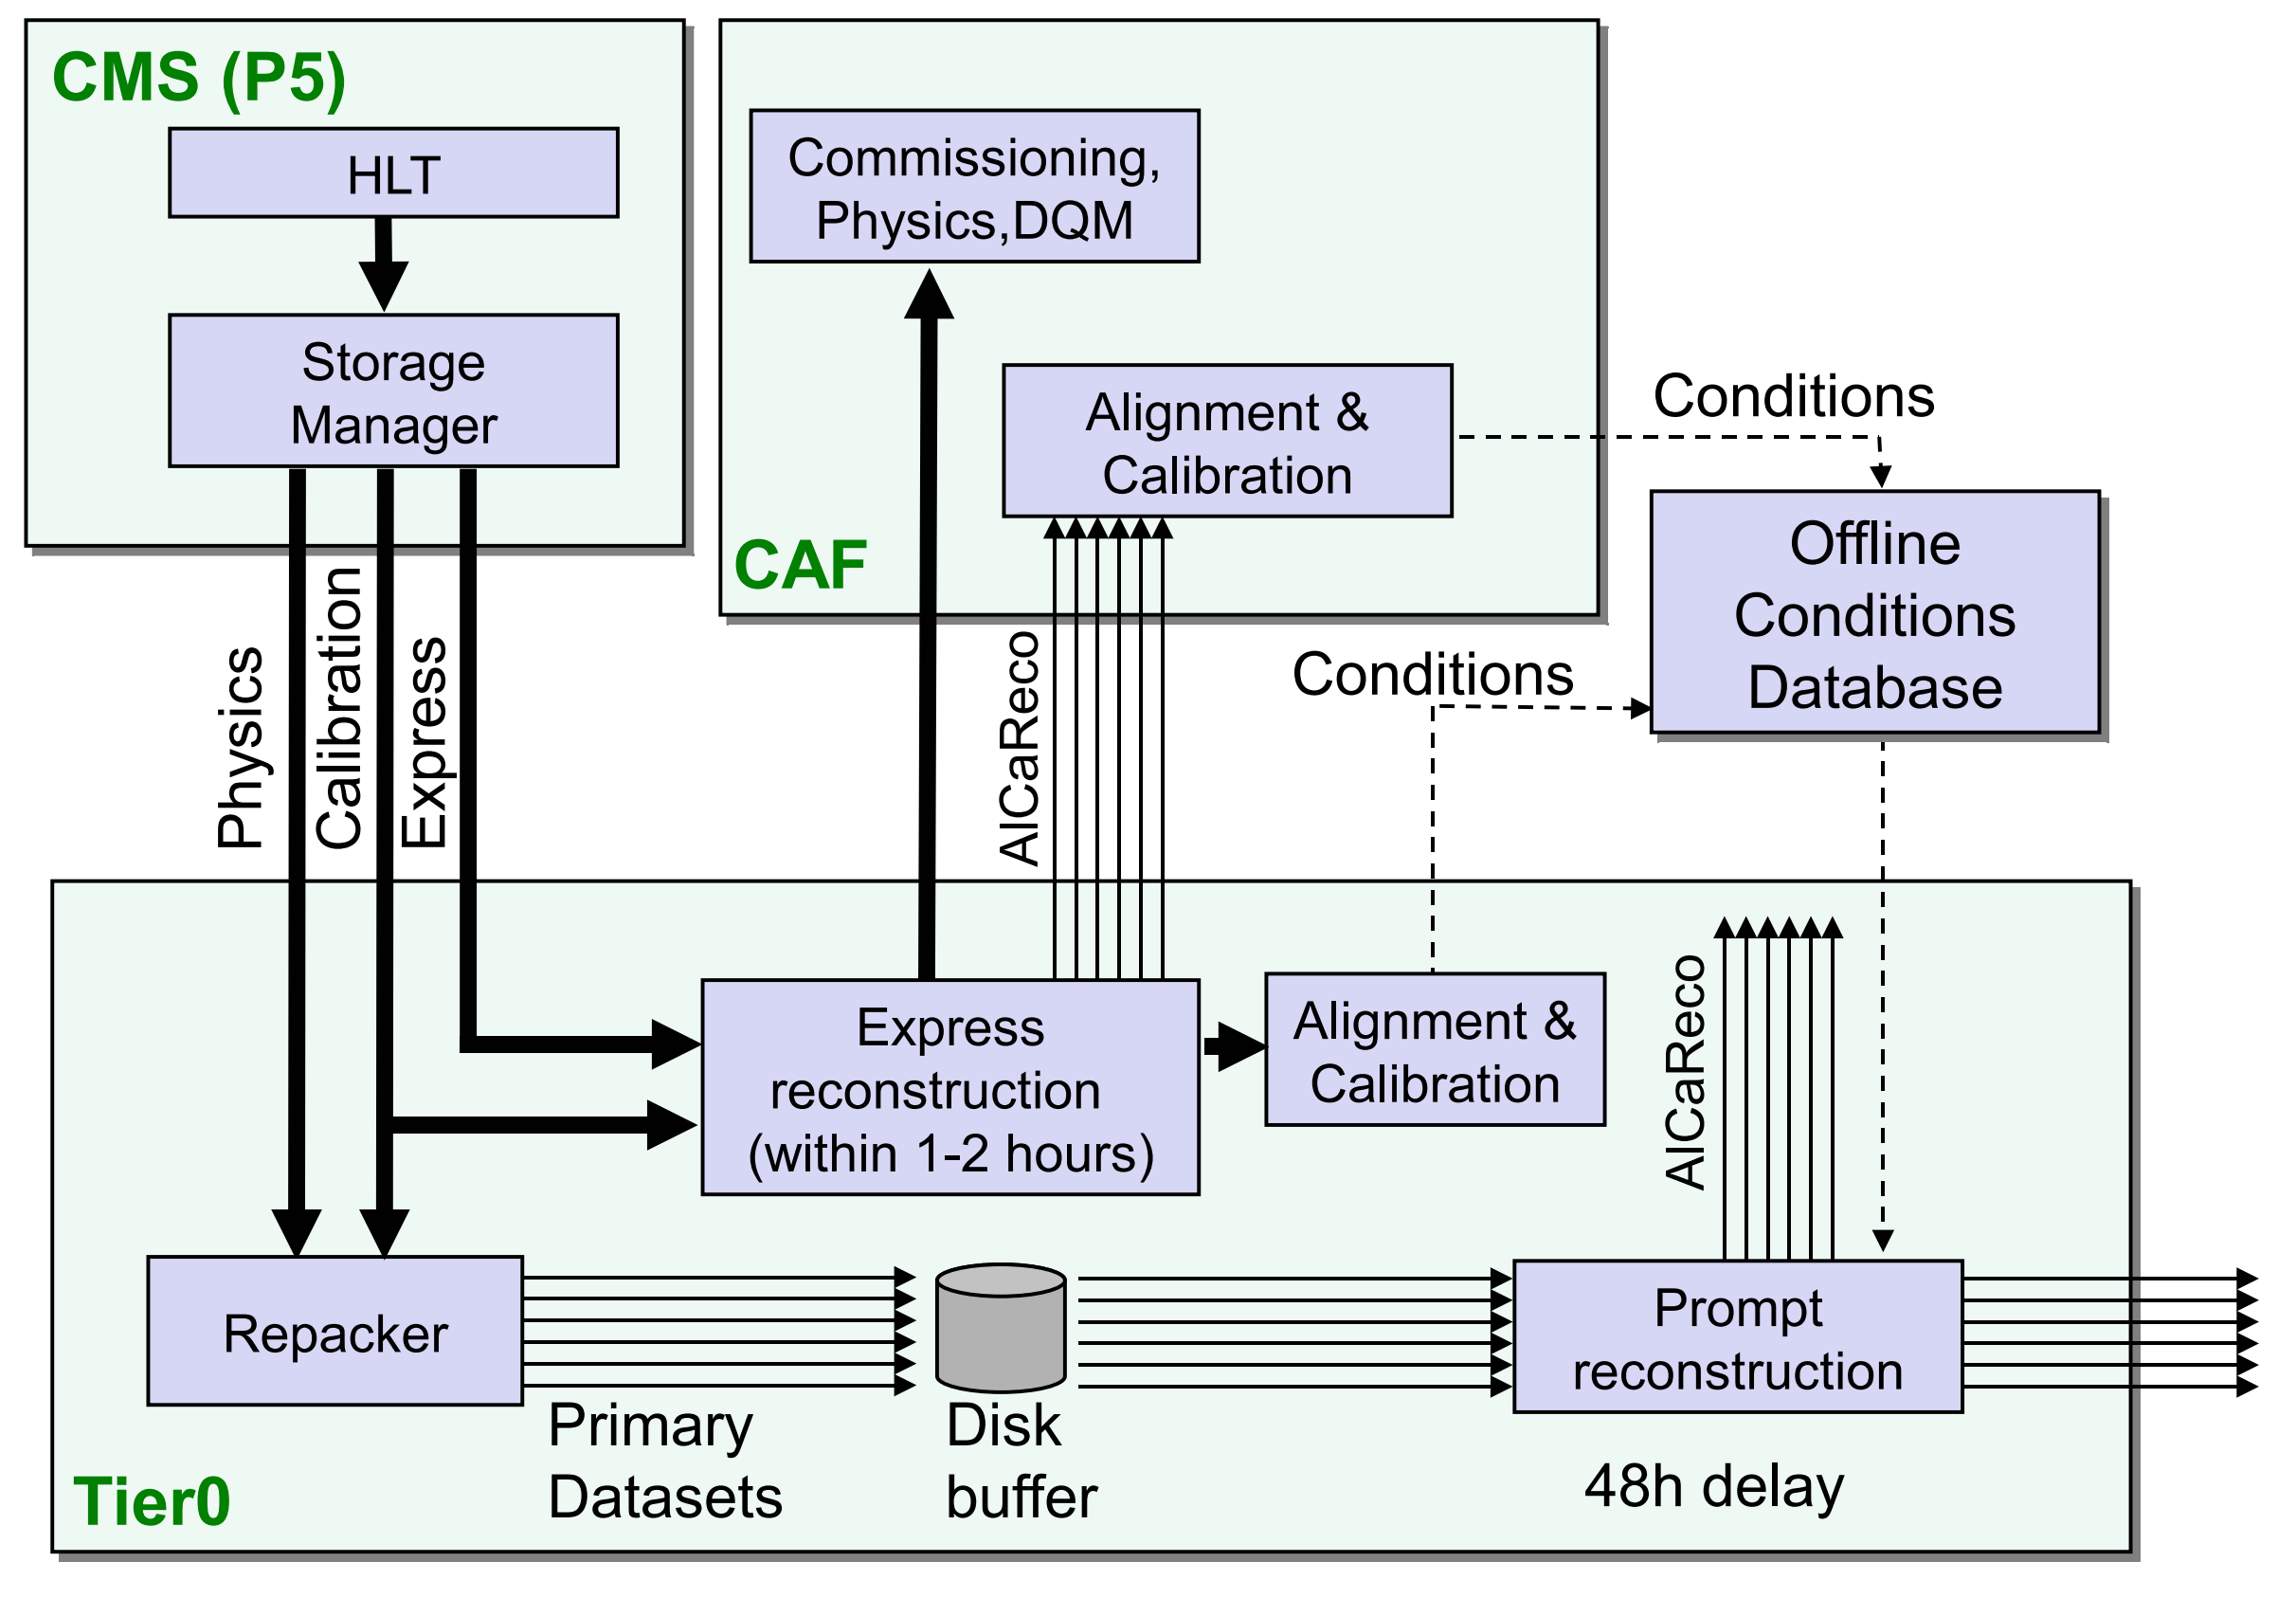
\includegraphics[width=0.75\textwidth]{figures/Tier0.png}    
    \caption{\label{fig:t0} Schematic overiew of Tier0 computing, data can be available from different sections allowing for data quality monitoring and also storage to several databases ~\cite{Hufnagel:1319049} }
\end{figure}

The data can then be stored at many different sites. The sites are demarcated based on importance and functionality. There is one Tier-0, seven Tier-1, about one-hundred fifty Tier-2, and numerous Tier-3 centers. The sum of these tiers is the ``grid'' or the Worldwide LHC Computing Grid (WLCG), which in total combines 900 000 cpus from over 170 sites in 42 countries. \texttt{XrootD} and tools like \texttt{Rucio} are used for a global file lookup service that allows physicists from around the world to access and use centrally supported data. An abundance of information that is constantly changing can be found \texttt{https://home.cern/science/computing/grid}. 



